\chapter{विषमचक्रीय रसायन}\label{ch:b3:heterocycles}

कॉफ़ी के एक प्याले में कैफ़ीन होता है, जो दो संगलित वलयों से बना है जिनमें चार
नाइट्रोजन परमाणु हैं, और इसकी सुगंध भूनने में बने दर्जनों फ़्यूरानों, पिरोलों, पाइराज़ीनों
और थायोफ़ीनों से आती है। किसी औषधालय की अलमारी की अधिकांश औषधियों में कम से कम
एक ऐसा वलय होता है जिसमें नाइट्रोजन, ऑक्सीजन या सल्फ़र परमाणु हो, और यही बात DNA के
क्षारकों, \omterm{def:b3:bioinorganic:haem}{हीम} और क्लोरोफ़िल, और अनेक विटामिनों पर भी लागू होती है। यह अध्याय समझाता है कि
किसी ऐरोमैटिक वलय में एक विषमपरमाणु उसके इलेक्ट्रॉनों को कैसे बदलता है: वह वलय को
बेंज़ीन से अधिक निर्धन या अधिक समृद्ध बना सकता है, और यही तय करता है कि वह कहाँ और
कैसे अभिक्रिया करता है। अध्याय ऐसे वलय बनाने की तीन क्लासिकी विधियों के साथ समाप्त होता है।

\begin{recall}
द्वितीय वर्ष के खंड ने ऐरोमैटिकता और ह्युकेल नियम, ऐरीन और व्हीलैंड मध्यवर्ती से होकर
इलेक्ट्रॉनरागी ऐरोमैटिक प्रतिस्थापन, सक्रियक और निर्देशक समूह, ऐमीन और उनकी क्षारकता, इमीन,
एनामीन, चलावयवी और न्यूक्लियोक्षारक प्रस्तुत किए; प्रथम वर्ष के खंड ने $\mathrm pK_a$, नाभिकरागी,
इलेक्ट्रॉनरागी और निर्गामी समूह। \Cref{ch:b3:pericyclic} ने [3,3]
\omterm{def:b3:pericyclic:families}{सिग्माट्रॉपी पुनर्विन्यास} दिया।
\end{recall}

\begin{omfigure}
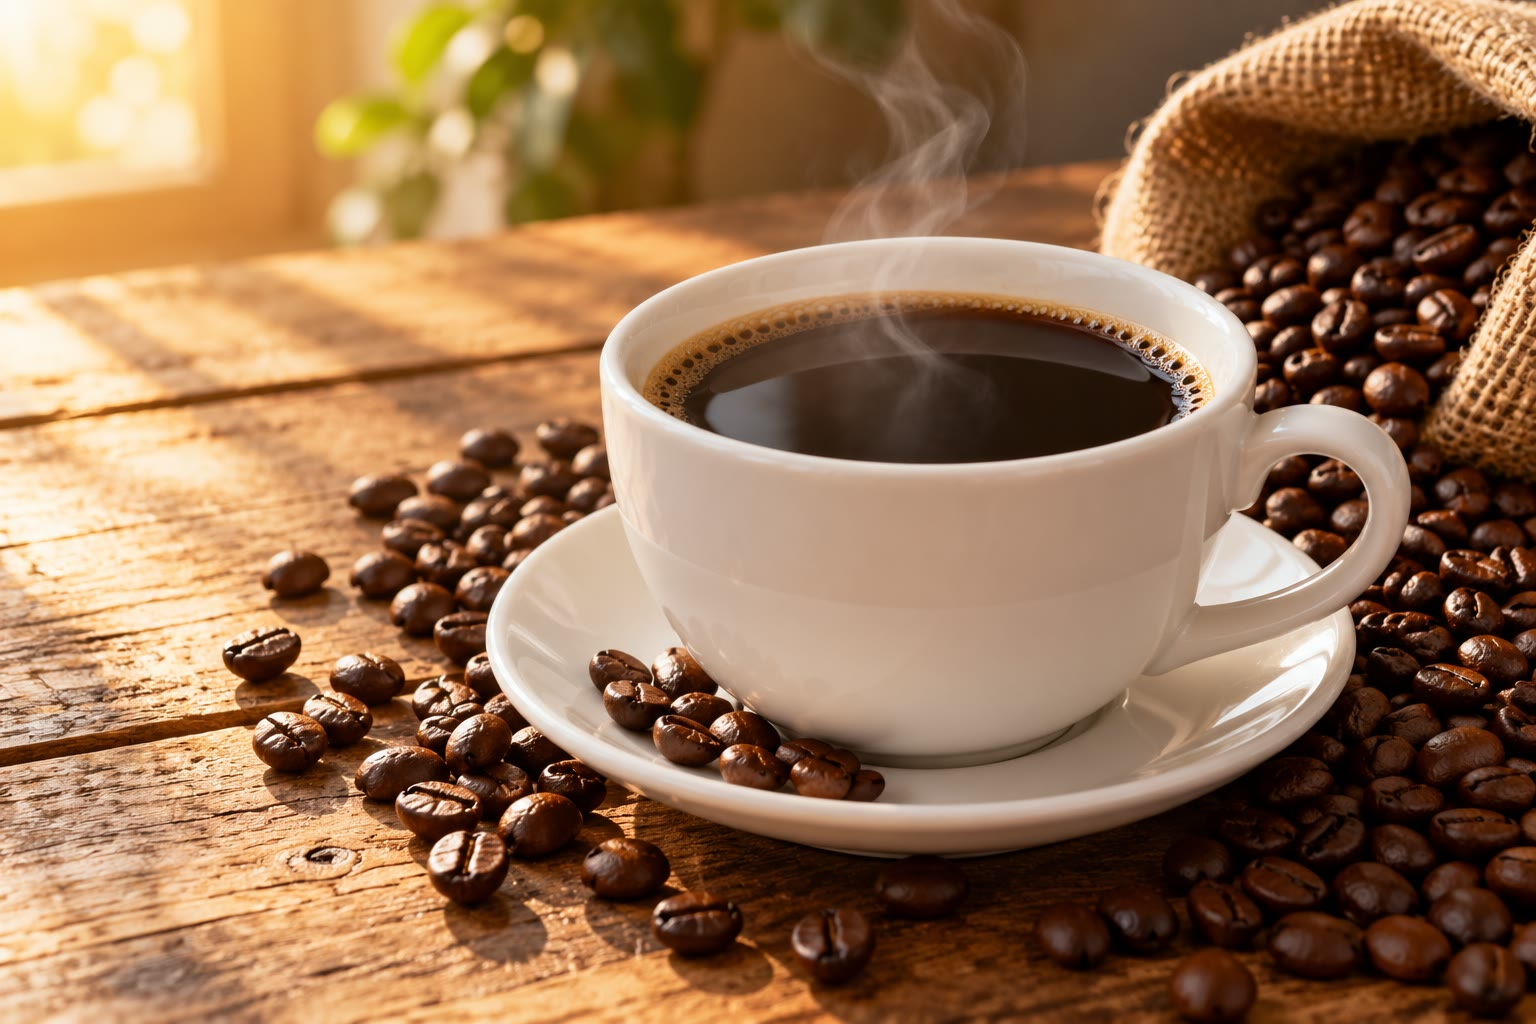
\includegraphics[width=0.5\linewidth]{images/book4/ai/b3-29-coffee.jpg}

{\small कॉफ़ी का एक प्याला और भुने हुए बीज: कैफ़ीन, एक प्यूरीन, और भूनने में बनने वाले
अनेक सुगंध-अणु \omterm{def:b3:heterocycles:heterocycle}{विषमचक्र} हैं।}
\end{omfigure}

\section{ऐरोमैटिक विषमचक्र}

\begin{definition}[विषमचक्र]\label{def:b3:heterocycles:heterocycle}
\emph{विषमचक्र}\index{विषमचक्र} ऐसा वलय-यौगिक है जिसके वलय में कार्बन के अतिरिक्त
कम से कम एक अन्य परमाणु हो; \emph{विषम-ऐरोमैटिक
यौगिक}\index{विषम-ऐरोमैटिक यौगिक} इनमें से ऐरोमैटिक यौगिक है, जैसे पिरिडीन,
पिरोल, फ़्यूरान या थायोफ़ीन।
\end{definition}

\begin{proposition}[छह $\pi$ इलेक्ट्रॉन]\label{prop:b3:heterocycles:sextet}
पिरिडीन, पिरोल, फ़्यूरान, थायोफ़ीन और इमिडाज़ोल प्रत्येक में एक समतलीय, चक्रीय, संयुग्मित
वलय में छह $\pi$ इलेक्ट्रॉन होते हैं, और ये ह्युकेल नियम से ऐरोमैटिक हैं।
\end{proposition}

\begin{proof}
पिरिडीन: पाँच कार्बन और नाइट्रोजन प्रत्येक एक p इलेक्ट्रॉन देते हैं; नाइट्रोजन का
एकाकी युग्म वलय-तल में स्थित एक $sp^2$ कक्षक में है, $\pi$ निकाय के बाहर: $5 + 1 = 6$।
पिरोल: चार कार्बन एक-एक देते हैं और नाइट्रोजन, जो तल में H से आबंधित है,
अपना एकाकी युग्म अपने p कक्षक में रखता है: $4 + 2 = 6$। फ़्यूरान और थायोफ़ीन: पिरोल की तरह,
विषमपरमाणु अपने दो एकाकी युग्मों में से एक देता है (दूसरा तल में स्थित है)। इमिडाज़ोल:
N--H नाइट्रोजन दो देता है, पिरिडीन-सदृश नाइट्रोजन एक, तीनों कार्बन
तीन: 6। छह $4n + 2$ है, जहाँ $n = 1$।
\end{proof}

\begin{omfigure}
\begin{tikzpicture}[font=\small, yscale=0.55]
  % pyridine: six p orbitals perpendicular to the ring (drawn first), N at 0 deg
  \foreach \a in {0,60,...,300} { \pic at (\a:1.1) {omp={0.62}{90}}; }
  \draw[thick] (0:1.1) -- (60:1.1) -- (120:1.1) -- (180:1.1) -- (240:1.1) -- (300:1.1) -- cycle;
  \node[fill=white, inner sep=0.5pt] at (0:1.1) {N};
  \pic at ($(0:1.1)+(0.2,0)$) {omlobe={0.8}{0}};
  \node[font=\scriptsize, align=center, anchor=north] at (0,-2.4) {पिरिडीन: 6 परमाणुओं से 6 p इलेक्ट्रॉन;\\ एकाकी युग्म तल में (क्षारीय)};
  \begin{scope}[xshift=5.4cm]
    \foreach \a in {0,72,144,216,288} { \pic at (\a:1.0) {omp={0.62}{90}}; }
    \draw[thick] (0:1.0) -- (72:1.0) -- (144:1.0) -- (216:1.0) -- (288:1.0) -- cycle;
    \node[fill=white, inner sep=0.5pt] at (0:1.0) {N};
    \draw ($(0:1.0)+(0.18,0)$) -- (0:1.7) node[right, inner sep=0.5pt] {H};
    \node[font=\scriptsize, align=center, anchor=north] at (0,-2.4) {पिरोल: N का एकाकी युग्म\\ 6 $\pi$ इलेक्ट्रॉनों का भाग है (क्षारीय नहीं)};
  \end{scope}
\end{tikzpicture}

{\small पिरिडीन और पिरोल के $\pi$ निकाय, तिरछे देखे गए: प्रति वलय-परमाणु एक p कक्षक,
वलय के लंबवत। पिरिडीन में नाइट्रोजन का एकाकी युग्म (तल में स्थित पालि, नाइट्रोजन पर)
वलय-तल में बाहर की ओर इंगित करता है और किसी प्रोटॉन को बाँधने के लिए मुक्त है; पिरोल में
नाइट्रोजन, जिस पर तल में एक हाइड्रोजन है, अपना एकाकी युग्म ऐरोमैटिक
षट्क को दे देता है।}
\end{omfigure}

\begin{definition}[$\pi$-अधिशेषी और $\pi$-न्यून विषमचक्र]\label{def:b3:heterocycles:pi-character}
\emph{$\pi$-अधिशेषी विषमचक्र}\index{पाई-अधिशेषी विषमचक्र@$\pi$-अधिशेषी विषमचक्र}, जैसे
पिरोल, फ़्यूरान या थायोफ़ीन, में पाँच परमाणुओं पर छह $\pi$ इलेक्ट्रॉन होते हैं और उसके
कार्बनों पर बेंज़ीन की तुलना में अधिक $\pi$ \omterm{def:b3:computational-chemistry:dft}{इलेक्ट्रॉन घनत्व} होता है; \emph{$\pi$-न्यून
विषमचक्र}\index{पाई-न्यून विषमचक्र@$\pi$-न्यून विषमचक्र}, जैसे पिरिडीन, में एक
विद्युतऋणी वलय-परमाणु होता है जो कार्बनों से $\pi$ घनत्व को दूर खींच लेता है।
\end{definition}

\begin{proposition}[क्षारकता]\label{prop:b3:heterocycles:basicity}
पिरिडीन एक मध्यम क्षारक है और पिरोल लगभग बिल्कुल नहीं; प्रबल अम्ल में
प्रोटॉनित होने पर पिरोल प्रोटॉन को नाइट्रोजन पर नहीं, कार्बन पर ग्रहण करता है।
\end{proposition}

\begin{proof}[तर्क]
% ledger: pka:pyridinium, pka4:pyrrolium, pka4:piperidinium, pka4:imidazolium, pka4:DMAPH
पिरिडीन का एकाकी युग्म $\pi$ निकाय के बाहर है: उसे प्रोटॉनित करने में कोई
ऐरोमैटिकता नहीं खोती, और पिरिडीनियम का $\mathrm pK_a = 5.2$ है; यह पिपेरिडीन से कम क्षारीय है
(पिरिडीनियम का नाइट्रोजन $sp^2$ है, अधिक s लक्षण के साथ, और अपने युग्म को अधिक
कसकर थामता है: पिपेरिडीनियम 11.1)। पिरोल के नाइट्रोजन को प्रोटॉनित करने से उसका एकाकी
युग्म षट्क से बाहर निकल जाता और ऐरोमैटिकता नष्ट हो जाती; केवल अति प्रबल अम्ल ही
पिरोल को प्रोटॉनित करते हैं, और वह भी C2 पर, जहाँ धनायन में कुछ विस्थानीकरण बना रहता है
($\mathrm pK_a$ लगभग $-4$)। इमिडाज़ोल में दोनों प्रकार के नाइट्रोजन हैं: वह
पिरिडीन-सदृश नाइट्रोजन पर प्रोटॉनित होता है, और उसका सममित धनायन अनुनाद से स्थायीकृत होता है ($\mathrm pK_a$
7.0), यही कारण है कि हिस्टिडीन \omterm{def:b3:complex-kinetics:enzyme}{एंज़ाइमों} में अम्ल और क्षारक दोनों के रूप में कार्य करता है।
4-(डाइमेथिलऐमीनो)पिरिडीन और भी अधिक क्षारीय है ($\mathrm pK_a$ 9.6): ऐमीनो समूह अपना
एकाकी युग्म वलय में और वलय-नाइट्रोजन पर धकेलता है।
\end{proof}

% ledger: dip:pyridine, dip4:pyrrole, dip4:furan, dip4:thiophene
द्विध्रुव आघूर्ण वही कहानी कहते हैं: पिरिडीन (\qty{2.19}{D}) का ऋण सिरा नाइट्रोजन पर
है, जबकि पिरोल (\qty{1.84}{D}) में एकाकी युग्म का वलय को दान ऋण सिरे को वलय पर
और धन सिरे को नाइट्रोजन पर रखता है। फ़्यूरान
(\qty{0.66}{D}) और थायोफ़ीन (\qty{0.55}{D}) में दोनों प्रभाव, $\sigma$ आकर्षण और $\pi$ दान, लगभग
एक-दूसरे को निरस्त कर देते हैं।

\begin{omfigure}
% ledger: h1:pyridine.a, h1:pyridine.g, h1:pyridine.b, h1:pyrrole.a, h1:pyrrole.b, h1:pyrrole.NH, h1:furan.a, h1:furan.b
\begin{tikzpicture}
\begin{axis}[width=0.86\linewidth, height=6.2cm, x dir=reverse, xmin=5.8, xmax=9.0, ymin=-0.1, ymax=3.6,
  axis x line=bottom, axis y line=none, xlabel={$\delta$ / ppm}, tick label style={font=\scriptsize}, label style={font=\small}]
\addplot[omDef, thick] table[x=ppm, y expr=\thisrow{y}+2.4] {figdata/out/bachelor-3-heterocycle-nmr-pyridine.dat};
\addplot[omThm, thick] table[x=ppm, y expr=\thisrow{y}+1.2] {figdata/out/bachelor-3-heterocycle-nmr-pyrrole.dat};
\addplot[omMeth, thick] table[x=ppm, y=y] {figdata/out/bachelor-3-heterocycle-nmr-furan.dat};
\node[font=\scriptsize, omDef, anchor=west] at (axis cs:7.1,3.0) {पिरिडीन: H2/6, H4, H3/5 (2\,:\,1\,:\,2)};
\node[font=\scriptsize, omThm, anchor=west] at (axis cs:7.7,1.8) {पिरोल: NH, H2/5, H3/4};
\node[font=\scriptsize, omMeth, anchor=west] at (axis cs:7.2,0.6) {फ़्यूरान: H2/5, H3/4};
\end{axis}
\end{tikzpicture}

{\small ड्यूटेरोक्लोरोफ़ॉर्म में पिरिडीन, पिरोल और फ़्यूरान का प्रोटॉन NMR, मापे गए
विस्थापनों से एकल रेखाओं के रूप में संश्लिष्ट (युग्मन छोड़ दिए गए), जिनके
क्षेत्रफल प्रोटॉनों की संख्याओं के बराबर हैं। $\pi$-न्यून पिरिडीन के H2/6 और H4
संकेत बेंज़ीन के संकेत से काफ़ी ऊँचे विस्थापन पर (डाउनफ़ील्ड) हैं; $\pi$-अधिशेषी पिरोल और फ़्यूरान
के अधिकांश संकेत उससे निचले विस्थापन पर (अपफ़ील्ड) हैं; विषमपरमाणु के बगल वाले प्रोटॉन सदैव
सबसे अधिक विपरिरक्षित होते हैं।}
\end{omfigure}

\section{पिरिडीन}

पिरिडीन इलेक्ट्रॉनरागी प्रतिस्थापन का प्रतिरोध करता है: इलेक्ट्रॉनरागी का सामना बेंज़ीन से
अधिक इलेक्ट्रॉन-निर्धन वलय से होता है, और, सामान्यतः उपस्थित अम्ल में, एक
पिरिडीनियम आयन से जिसका धन आवेश उसे प्रतिकर्षित करता है। नाइट्रीकरण के लिए अत्यंत कठोर
परिस्थितियाँ चाहिए और यह अल्प लब्धि में 3-समावयवी देता है।

\begin{proposition}[C3 पर इलेक्ट्रॉनरागी प्रतिस्थापन]\label{prop:b3:heterocycles:pyridine-c3}
पिरिडीन पर इलेक्ट्रॉनरागी आक्रमण C3 पर होता है: C2 या C4 पर आक्रमण ऐसा
व्हीलैंड मध्यवर्ती देता है जिसकी एक अनुनादी संरचना धन आवेश को ऐसे नाइट्रोजन
पर रखती है जिसके चारों ओर केवल छह इलेक्ट्रॉन हैं।
\end{proposition}

\begin{proof}
C2 (या C4) पर आक्रमण से बने धनायन में धन आवेश C3, C5
और N1 (या C3, C5 और N1) पर फैला होता है: एक इलेक्ट्रॉन-न्यून, छह-इलेक्ट्रॉन
नाइट्रोजन वाली अनुनादी संरचना, जो किसी विद्युतऋणी परमाणु के लिए अत्यंत प्रतिकूल है। C3 पर
आक्रमण आवेश को केवल C2, C4 और C6 पर फैलाता है। तीनों धनायन बेंज़ीन के धनायन से कम
स्थायी हैं, परंतु C3 आक्रमण सबसे कम बुरा है।
\end{proof}

\begin{definition}[पिरिडीन N-ऑक्साइड]\label{def:b3:heterocycles:n-oxide}
\emph{पिरिडीन N-ऑक्साइड}\index{पिरिडीन N-ऑक्साइड}, जो पिरिडीन को किसी पेरॉक्सी अम्ल से
ऑक्सीकृत करके बनाया जाता है, में एक $\mathrm{N^+{-}O^-}$ समूह होता है जिसका ऑक्सीजन C2
और C4 को इलेक्ट्रॉन वापस देता है; इसमें C4 पर इलेक्ट्रॉनरागी प्रतिस्थापन होता है, और फिर
ऑक्सीजन हटा दिया जाता है।
\end{definition}

\begin{definition}[नाभिकरागी ऐरोमैटिक प्रतिस्थापन]\label{def:b3:heterocycles:snar}
\emph{नाभिकरागी ऐरोमैटिक प्रतिस्थापन}\index{नाभिकरागी ऐरोमैटिक प्रतिस्थापन}
($\mathrm S_\mathrm NAr$) किसी इलेक्ट्रॉन-निर्धन ऐरोमैटिक वलय पर स्थित निर्गामी समूह को
एक नाभिकरागी से प्रतिस्थापित करता है, योग और उसके बाद विलोपन से होकर। ऋणायनी
योग मध्यवर्ती एक \emph{माइज़नहाइमर संकुल}\index{माइज़नहाइमर संकुल} है।
\end{definition}

\begin{proposition}[C2 और C4 पर $\mathrm S_\mathrm NAr$]\label{prop:b3:heterocycles:snar-positions}
हैलोपिरिडीनों में C2 और C4 पर $\mathrm S_\mathrm NAr$ सरलता से होता है और C3 पर केवल मंद गति से,
क्योंकि C2 या C4 पर योग ऋण आवेश को नाइट्रोजन पर रखता है।
\end{proposition}

\begin{proof}
C2 पर योग C2 को $sp^3$ बना देता है और चार $\pi$ इलेक्ट्रॉनों तथा आने वाले युग्म को
N1, C3 और C5 पर (या C4 के लिए: C3, C5 और N1 पर) फैला छोड़ता है: एक अनुनादी संरचना में
ऋण आवेश विद्युतऋणी नाइट्रोजन पर होता है। C3 पर योग इसे केवल
C2, C4 और C6 पर फैलाता है, जो सभी कार्बन हैं।
\end{proof}

\begin{omfigure}
\begin{tikzpicture}[font=\small, >=Stealth]
  \draw[thick] (-0.000,-0.620) -- (0.537,-0.310) -- (0.537,0.310) -- (0.000,0.620) -- (-0.537,0.310) -- (-0.537,-0.310) -- cycle;
  \draw[thick] (0.082,-0.424) -- (0.326,-0.283);
  \draw[thick] (0.326,0.283) -- (0.082,0.424);
  \draw[thick] (-0.408,0.141) -- (-0.408,-0.141);
  \node[fill=white, inner sep=0.4pt, font=\scriptsize] at (-0.000,-0.620) {N};
  \draw (0.537,-0.310) -- (0.927,-0.535) node[right, inner sep=0.5pt, font=\scriptsize] {Cl};
  \draw[thick] (3.400,-0.620) -- (3.937,-0.310) -- (3.937,0.310) -- (3.400,0.620) -- (2.863,0.310) -- (2.863,-0.310) -- cycle;
  \draw[thick] (3.726,0.283) -- (3.482,0.424);
  \draw[thick] (2.992,0.141) -- (2.992,-0.141);
  \node[fill=white, inner sep=0.4pt, font=\scriptsize] at (3.400,-0.620) {N};
  \node[font=\scriptsize, omThm] at (3.350,-0.920) {$\ominus$};
  \draw (3.937,-0.310) -- (4.386,-0.343) node[right, inner sep=0.5pt, font=\scriptsize] {Nu};
  \draw (3.937,-0.310) -- (4.190,-0.682) node[right, inner sep=0.5pt, font=\scriptsize] {Cl};
  \draw[thick] (6.800,-0.620) -- (7.337,-0.310) -- (7.337,0.310) -- (6.800,0.620) -- (6.263,0.310) -- (6.263,-0.310) -- cycle;
  \draw[thick] (6.882,-0.424) -- (7.126,-0.283);
  \draw[thick] (7.126,0.283) -- (6.882,0.424);
  \draw[thick] (6.392,0.141) -- (6.392,-0.141);
  \node[fill=white, inner sep=0.4pt, font=\scriptsize] at (6.800,-0.620) {N};
  \draw (7.337,-0.310) -- (7.727,-0.535) node[right, inner sep=0.5pt, font=\scriptsize] {Nu};
  \draw[->, thick] (1.25,0) -- (2.35,0) node[midway, above, font=\scriptsize] {$+\,\mathrm{Nu^-}$};
  \draw[->, thick] (4.65,0) -- (5.75,0) node[midway, above, font=\scriptsize] {$-\,\ce{Cl-}$};
  \node[font=\scriptsize] at (3.4,-1.2) {माइज़नहाइमर संकुल};
\end{tikzpicture}

{\small 2-क्लोरोपिरिडीन का नाभिकरागी प्रतिस्थापन: नाभिकरागी C2 पर जुड़ता है,
जिससे एक ऋणायनी मध्यवर्ती बनता है जिसका ऋण आवेश मुख्यतः वलय-नाइट्रोजन पर होता है
(एक अनुनादी संरचना दर्शाई गई है); फिर क्लोराइड निकल जाता है और
ऐरोमैटिक वलय पुनः स्थापित हो जाता है।}
\end{omfigure}

\begin{proposition}[योग--विलोपन]\label{prop:b3:heterocycles:snar-mechanism}
जिस $\mathrm S_\mathrm NAr$ अभिक्रिया का योग चरण दर-निर्धारक हो, उसके लिए $v = k[\mathrm{ArX}][\mathrm{Nu^-}]$,
और फ़्लुओराइड सबसे अच्छा हैलाइड निर्गामी समूह है।
\end{proposition}

\begin{proof}[तर्क]
दर द्विअणुक योग की दर है। उस चरण में कार्बन--हैलोजन आबंध नहीं
टूटता; महत्त्व इस बात का है कि हैलोजन इलेक्ट्रॉनों को आकर्षित करके ऋणायनी संक्रमण अवस्था
की ऊर्जा को कितना घटाता है, और सबसे अधिक विद्युतऋणी फ़्लुओरीन ऐसा सबसे अधिक
करता है: क्रम F $>$ Cl $\approx$ Br $>$ I है, जो $\mathrm S_\mathrm N2$ के क्रम के विपरीत है।
\end{proof}

\begin{definition}[चिचिबाबिन अभिक्रिया]\label{def:b3:heterocycles:chichibabin}
\emph{चिचिबाबिन अभिक्रिया}\index{चिचिबाबिन अभिक्रिया} सोडियम ऐमाइड द्वारा पिरिडीन का
C2 पर ऐमीनन है: ऐमाइड आयन C2 पर जुड़ता है, और एक हाइड्राइड आयन निकलता है, जो
उत्पाद से अभिक्रिया के बाद डाइहाइड्रोजन के रूप में मुक्त होता है।
\end{definition}

पिरिडीन और DMAP क्षारकों और नाभिकरागी उत्प्रेरकों के रूप में भी काम करते हैं: अम्ल
ऐनहाइड्राइडों के साथ ऐसिलनों में DMAP पहले ऐनहाइड्राइड पर आक्रमण करता है, जिससे एक
ऐसिलपिरिडीनियम आयन बनता है जो अपना ऐसिल समूह ऐल्कोहॉल को स्वयं
ऐनहाइड्राइड की तुलना में कहीं तेज़ी से स्थानांतरित करता है। पिरिडीन, बाइपिरिडीन और फ़ेनैन्थ्रोलीन
उपसहसंयोजन रसायन के सबसे सामान्य लिगैंडों में हैं।

\section{पंचसदस्यीय वलय}

\begin{proposition}[C2 पर पिरोल का इलेक्ट्रॉनरागी प्रतिस्थापन]\label{prop:b3:heterocycles:pyrrole-c2}
पिरोल, फ़्यूरान और थायोफ़ीन में इलेक्ट्रॉनरागी प्रतिस्थापन मुख्यतः C2 पर होता है,
क्योंकि C2 पर आक्रमण से बने धनायन की तीन अनुनादी संरचनाएँ होती हैं और C3 पर
आक्रमण से बने धनायन की केवल दो।
\end{proposition}

\begin{proof}
C2 पर आक्रमण के बाद धन आवेश C3 पर, C5 पर, या नाइट्रोजन पर रह सकता है,
जहाँ वह एकाकी युग्म के माध्यम से साझा होता है और प्रत्येक परमाणु अपना अष्टक बनाए रखता है (तीसरी
संरचना)। C3 पर आक्रमण के बाद वह केवल C2 पर या नाइट्रोजन पर रह सकता है: आवेश
का विस्थानीकरण कम होता है (चित्र देखिए)।
\end{proof}

\begin{omfigure}
\begin{tikzpicture}[font=\small]
  \draw[thick] (0.000,0.620) -- (0.590,0.192) -- (0.364,-0.502) -- (-0.364,-0.502) -- (-0.590,0.192) -- cycle;
  \draw[thick] (-0.303,-0.269) -- (-0.403,0.039);
  \node[fill=white, inner sep=0.4pt, font=\scriptsize] at (0.000,0.620) {N};
  \draw (0.000,0.750) -- (0.000,1.020) node[above, inner sep=0.5pt, font=\scriptsize] {H};
  \draw (0.590,0.192) -- (0.893,0.482) node[right, inner sep=0.5pt, font=\scriptsize] {H};
  \draw (0.590,0.192) -- (1.006,0.135) node[right, inner sep=0.5pt, font=\scriptsize] {E};
  \node[font=\scriptsize, omThm] at (0.164,-0.226) {$\oplus$};
  \draw[thick] (2.600,0.620) -- (3.190,0.192) -- (2.964,-0.502) -- (2.236,-0.502) -- (2.010,0.192) -- cycle;
  \draw[thick] (2.762,-0.371) -- (2.438,-0.371);
  \node[fill=white, inner sep=0.4pt, font=\scriptsize] at (2.600,0.620) {N};
  \draw (2.600,0.750) -- (2.600,1.020) node[above, inner sep=0.5pt, font=\scriptsize] {H};
  \draw (3.190,0.192) -- (3.493,0.482) node[right, inner sep=0.5pt, font=\scriptsize] {H};
  \draw (3.190,0.192) -- (3.606,0.135) node[right, inner sep=0.5pt, font=\scriptsize] {E};
  \node[font=\scriptsize, omThm] at (2.335,0.086) {$\oplus$};
  \draw[thick] (5.200,0.620) -- (5.790,0.192) -- (5.564,-0.502) -- (4.836,-0.502) -- (4.610,0.192) -- cycle;
  \draw[thick] (5.362,-0.371) -- (5.038,-0.371);
  \draw[thick] (5.113,0.395) -- (4.851,0.205);
  \node[fill=white, inner sep=0.4pt, font=\scriptsize] at (5.200,0.620) {N};
  \draw (5.200,0.750) -- (5.200,1.020) node[above, inner sep=0.5pt, font=\scriptsize] {H};
  \draw (5.790,0.192) -- (6.093,0.482) node[right, inner sep=0.5pt, font=\scriptsize] {H};
  \draw (5.790,0.192) -- (6.206,0.135) node[right, inner sep=0.5pt, font=\scriptsize] {E};
  \node[font=\scriptsize, omThm] at (5.480,0.700) {$\oplus$};
  \draw[thick] (8.400,0.620) -- (8.990,0.192) -- (8.764,-0.502) -- (8.036,-0.502) -- (7.810,0.192) -- cycle;
  \draw[thick] (8.097,-0.269) -- (7.997,0.039);
  \node[fill=white, inner sep=0.4pt, font=\scriptsize] at (8.400,0.620) {N};
  \draw (8.400,0.750) -- (8.400,1.020) node[above, inner sep=0.5pt, font=\scriptsize] {H};
  \draw (8.764,-0.502) -- (9.135,-0.700) node[right, inner sep=0.5pt, font=\scriptsize] {H};
  \draw (8.764,-0.502) -- (8.839,-0.915) node[right, inner sep=0.5pt, font=\scriptsize] {E};
  \node[font=\scriptsize, omThm] at (8.665,0.086) {$\oplus$};
  \draw[thick] (11.000,0.620) -- (11.590,0.192) -- (11.364,-0.502) -- (10.636,-0.502) -- (10.410,0.192) -- cycle;
  \draw[thick] (10.697,-0.269) -- (10.597,0.039);
  \draw[thick] (11.087,0.395) -- (11.349,0.205);
  \node[fill=white, inner sep=0.4pt, font=\scriptsize] at (11.000,0.620) {N};
  \draw (11.000,0.750) -- (11.000,1.020) node[above, inner sep=0.5pt, font=\scriptsize] {H};
  \draw (11.364,-0.502) -- (11.735,-0.700) node[right, inner sep=0.5pt, font=\scriptsize] {H};
  \draw (11.364,-0.502) -- (11.439,-0.915) node[right, inner sep=0.5pt, font=\scriptsize] {E};
  \node[font=\scriptsize, omThm] at (11.280,0.700) {$\oplus$};
  \node[font=\scriptsize] at (2.6,-1.35) {C2 पर आक्रमण: तीन संरचनाएँ};
  \node[font=\scriptsize] at (9.7,-1.35) {C3 पर आक्रमण: दो संरचनाएँ};
  \draw[black!40] (6.8,-1.2) -- (6.8,1.2);
\end{tikzpicture}

{\small पिरोल के व्हीलैंड मध्यवर्ती (E: इलेक्ट्रॉनरागी; $\oplus$: धन आवेश)।
C2 पर आक्रमण ऐसा धनायन देता है जिसमें आवेश C3 पर, C5 पर, या सभी अष्टक पूर्ण
रखते हुए नाइट्रोजन पर होता है; C3 पर आक्रमण, केवल C2 या नाइट्रोजन पर।}
\end{omfigure}

पिरोल लगभग फ़ीनॉल या ऐनिलीन जितना अभिक्रियाशील है: इसका ब्रोमीनन, नाइट्रीकरण
और ऐसिलन मृदु परिस्थितियों में होता है, प्रबल अम्ल में यह बहुलकित हो जाता है, और
डाइमेथिलफ़ॉर्मामाइड तथा फ़ॉस्फ़ोरिल क्लोराइड से बने विल्समायर अभिकर्मक द्वारा C2 पर इसका
फ़ॉर्मिलन होता है। अभिक्रियाशीलताएँ पिरोल $>$ फ़्यूरान $>$ थायोफ़ीन $>$ बेंज़ीन क्रम में घटती हैं,
विषमपरमाणु की अपना एकाकी युग्म साझा करने की तत्परता के अनुसार। सबसे कम ऐरोमैटिक
फ़्यूरान डील्स--ऐल्डर अभिक्रियाओं में डाईन के रूप में भी अभिक्रिया करता है। ब्यूटिललिथियम
जैसे प्रबल क्षारक फ़्यूरान और थायोफ़ीन को विषमपरमाणु के बगल में C2 पर
विप्रोटॉनित करते हैं, जिससे कार्बलिथियम अभिकर्मक बनते हैं।

\begin{method}[किसी विषमचक्र पर आक्रमण-स्थल का पूर्वानुमान]\label{met:b3:heterocycles:site}
\begin{enumerate}
  \item वलय का वर्गीकरण कीजिए: $\pi$-अधिशेषी (पिरोल-सदृश विषमपरमाणु) या $\pi$-न्यून
        (पिरिडीन-सदृश नाइट्रोजन)।
  \item इलेक्ट्रॉनरागी: $\pi$-अधिशेषी वलय पर C2 पर (इंडोल के लिए C3 पर, क्योंकि उसमें C2 आक्रमण
        बेंज़ीन वलय को भंग कर देता); पिरिडीन पर C3 पर, या
        N-ऑक्साइड के माध्यम से C4 पर।
  \item नाभिकरागी: $\pi$-न्यून वलय पर C2 या C4 पर, विशेषकर जब वहाँ कोई निर्गामी
        समूह हो।
  \item प्रबल क्षारक: विषमपरमाणु के बगल वाले C--H पर।
\end{enumerate}
\end{method}

\section{संगलित और जैविक विषमचक्र}

इंडोल, पिरोल से संगलित एक बेंज़ीन, इलेक्ट्रॉनरागियों से C3 पर अभिक्रिया करता है: वहाँ
मध्यवर्ती बेंज़ीन वलय को अक्षुण्ण रखता है, और आवेश नाइट्रोजन पर होता है।
क्विनोलीन, पिरिडीन से संगलित एक बेंज़ीन, में इलेक्ट्रॉनरागी प्रतिस्थापन उसके
बेंज़ीन वलय पर और नाभिकरागी प्रतिस्थापन C2 और C4 पर होता है। न्यूक्लियोक्षारक
पिरिमिडीन (साइटोसीन, थाइमीन, यूरेसिल) और प्यूरीन (ऐडेनीन, ग्वानीन) हैं, जहाँ प्यूरीन
इमिडाज़ोल से संगलित एक पिरिमिडीन है। उनके ऑक्सो और ऐमीनो रूप (लैक्टम और ऐमीन
चलावयवी) हाइड्रॉक्सी और इमीनो रूपों पर हावी रहते हैं, जो प्रत्येक क्षारक पर
हाइड्रोजन-आबंध दाताओं और ग्राहियों का प्रतिरूप तय करता है, और इस प्रकार क्षारक युग्मन।

\begin{omfigure}
\begin{tikzpicture}[font=\small]
  \node[draw, rounded corners, minimum width=1.8cm, minimum height=2.8cm, fill=omDef!8] at (0,0) {};
  \node[font=\small\bfseries] at (0,1.75) {ग्वानीन};
  \node[anchor=east] (g1) at (0.85,0.85) {C6=O};
  \node[anchor=east] (g2) at (0.85,0) {N1--H};
  \node[anchor=east] (g3) at (0.85,-0.85) {C2--N--H};
  \node[draw, rounded corners, minimum width=1.8cm, minimum height=2.8cm, fill=omThm!8] at (3.2,0) {};
  \node[font=\small\bfseries] at (3.2,1.75) {साइटोसीन};
  \node[anchor=west] (c1) at (2.35,0.85) {H--N--C4};
  \node[anchor=west] (c2) at (2.35,0) {N3};
  \node[anchor=west] (c3) at (2.35,-0.85) {O=C2};
  \draw[omMeth, very thick, dotted] (g1.east) -- (c1.west);
  \draw[omMeth, very thick, dotted] (g2.east) -- (c2.west);
  \draw[omMeth, very thick, dotted] (g3.east) -- (c3.west);
\end{tikzpicture}

{\small एक ग्वानीन--साइटोसीन क्षारक युग्म, व्यवस्थात्मक: तीन हाइड्रोजन आबंध (हरे),
ग्वानीन के कार्बोनिल ऑक्सीजन और साइटोसीन के एक ऐमीनो N--H के बीच, ग्वानीन के N1--H
और साइटोसीन के वलय N3 के बीच, और ग्वानीन के एक ऐमीनो N--H और साइटोसीन के
कार्बोनिल ऑक्सीजन के बीच। ऐडेनीन और थाइमीन दो बनाते हैं।}
\end{omfigure}

\section{वलय बनाना}

\begin{definition}[पाल--नॉर संश्लेषण]\label{def:b3:heterocycles:paal-knorr}
\emph{पाल--नॉर संश्लेषण}\index{पाल--नॉर संश्लेषण} किसी 1,4-डाइकार्बोनिल यौगिक से
एक फ़्यूरान (अम्ल के साथ), एक पिरोल (किसी प्राथमिक ऐमीन या अमोनिया के साथ) या एक
थायोफ़ीन (किसी सल्फ़र अभिकर्मक के साथ) बनाता है।
\end{definition}

\begin{definition}[हांत्श पिरिडीन संश्लेषण]\label{def:b3:heterocycles:hantzsch}
\emph{हांत्श पिरिडीन संश्लेषण}\index{हांत्श पिरिडीन संश्लेषण} एक ऐल्डिहाइड, किसी
$\beta$-कीटो एस्टर के दो तुल्यांक और अमोनिया को संघनित करके एक
1,4-डाइहाइड्रोपिरिडीन बनाता है, जिसे पिरिडीन में ऑक्सीकृत किया जा सकता है।
\end{definition}

\begin{definition}[फ़िशर इंडोल संश्लेषण]\label{def:b3:heterocycles:fischer-indole}
\emph{फ़िशर इंडोल संश्लेषण}\index{फ़िशर इंडोल संश्लेषण} किसी ऐल्डिहाइड या कीटोन के
फ़ेनिलहाइड्रैज़ोन को एक अम्ल उत्प्रेरक के साथ गर्म करता है: हाइड्रैज़ोन चलावयवन द्वारा
एक ईन-हाइड्रैज़ीन में बदल जाता है, जिसमें [3,3] \omterm{def:b3:pericyclic:families}{सिग्माट्रॉपी
पुनर्विन्यास} होता है; चक्रीकरण और अमोनिया का निकास इंडोल देते हैं।
\end{definition}

\begin{omfigure}
\setchemfig{atom sep=1.8em}
\schemestart
\chemfig{*6(-=-=(-NH-[:30]N=[:-30](-[:-90]CH_3)-[:30]CH_3)-=)}
\arrow{->[$\ce{H+}$][चलावयवन]}[,1.4]
\chemfig{*6(-=-=(-NH-[:30]NH-[:-30](=[:-90]CH_2)-[:30]CH_3)-=)}
\schemestop
\par\bigskip
\schemestart
\arrow{->[{[3,3]}, फिर][चक्रीकरण, $-\ce{NH3}$]}[,2.2]
\chemfig{*6(-=*5(-=(-CH_3)-N(-H)-)-=-=)}
\schemestop

{\small ऐसीटोन फ़ेनिलहाइड्रैज़ोन से \omterm{def:b3:heterocycles:fischer-indole}{फ़िशर इंडोल संश्लेषण}। अम्ल
हाइड्रैज़ोन को उसके ईन-हाइड्रैज़ीन चलावयवी में बदलता है; [3,3] पुनर्विन्यास
N--N आबंध को तोड़ता है और नाइट्रोजन के \textit{ऑर्थो} वलय-कार्बन तथा
अंतस्थ $\ce{CH2}$ के बीच एक C--C आबंध बनाता है; नया ऐमीन इमीन पर आक्रमण करता है, और
अमोनिया का निकास 2-मेथिलइंडोल देता है।}
\end{omfigure}

\begin{method}[किसी विषमचक्र का विच्छेदन]\label{met:b3:heterocycles:disconnect}
\begin{enumerate}
  \item 2,5-द्विप्रतिस्थापित पिरोल, फ़्यूरान या थायोफ़ीन: विषमपरमाणु से जुड़े दोनों
        आबंधों का विच्छेदन कीजिए, और 1,4-डाइकीटोन पर लौटिए (पाल--नॉर)।
  \item C3 और C5 पर एस्टर वाला एक सममित 1,4-डाइहाइड्रोपिरिडीन: एक
        ऐल्डिहाइड, दो $\beta$-कीटो एस्टर और अमोनिया पर लौटिए (हांत्श)।
  \item 2,3-द्विप्रतिस्थापित इंडोल: फ़ेनिलहाइड्रैज़ीन और कीटोन
        $\mathrm{R^2CH_2COR^3}$ पर लौटिए (फ़िशर)।
  \item टुकड़ों की उपलब्धता जाँचिए, फिर, कीटोन के असममित होने पर,
        स्थान-रसायन।
\end{enumerate}
\end{method}

\begin{definition}[जैवसमरूपक]\label{def:b3:heterocycles:bioisostere}
\emph{जैवसमरूपक}\index{जैवसमरूपक} वह समूह है जो किसी औषध अणु में दूसरे समूह का
स्थान लेते हुए उसकी जैविक सक्रियता बनाए रखता है, क्योंकि उसका आकार, आकृति
और हाइड्रोजन-आबंधन तथा आवेश का प्रतिरूप समान होता है, जैसे कार्बोक्सिलिक अम्ल के
स्थान पर एक टेट्राज़ोल, या बेंज़ीन वलय के स्थान पर एक पिरिडीन।
\end{definition}

\begin{inthelab}[एक पाल--नॉर पिरोल]
हेक्सेन-2,5-डाइओन, ऐनिलीन और उत्प्रेरकी मात्रा में 4-टॉलूईनसल्फ़ोनिक अम्ल को
डीन--स्टार्क पात्र लगे फ़्लास्क में टॉलूईन में पश्चवाह के अधीन गर्म किया जाता है: बना हुआ
जल स्थिरक्वाथी के रूप में ऊपर जाकर पार्श्व भुजा में एकत्र होता है, जो
संघनन को पूर्णता तक ले जाता है। जब और जल पृथक नहीं होता, तो
विलयन को जलीय सोडियम हाइड्रोजनकार्बोनेट से धोया, शुष्क किया और वाष्पित किया जाता है,
और 2,5-डाइमेथिल-1-फ़ेनिलपिरोल का पुनःक्रिस्टलन किया जाता है।
\end{inthelab}

\begin{safety}{\ghs[0.62cm]{GHS02}\ghs[0.62cm]{GHS06}\ghs[0.62cm]{GHS07}\ghs[0.62cm]{GHS08}\ghs[0.62cm]{GHS09}}
% ledger: ghs4:pyridine, ghs4:phenylhydrazine
पिरिडीन: अत्यधिक ज्वलनशील, सभी मार्गों से हानिकारक, तीव्र गंध वाला; धूम-हुड में
प्रयुक्त। फ़ेनिलहाइड्रैज़ीन: सभी मार्गों से विषैला, कैंसर और आनुवंशिक दोष उत्पन्न कर सकता है,
बार-बार संपर्क से रक्त को क्षति पहुँचाता है, संवेदीकारक, जलीय जीवों के लिए अत्यधिक
विषैला; इसे दस्तानों के साथ धूम-हुड में तौला जाता है, और इसका अपशिष्ट
अलग एकत्र किया जाता है।
\end{safety}

\begin{history}[दो क्लासिकी वलय-संश्लेषण]
एमिल फ़िशर ने अपने इंडोल संश्लेषण का वर्णन 1883 में किया, उन्हीं वर्षों में जब वे
शर्कराओं और प्यूरीनों पर कार्य कर रहे थे; आर्थर हांत्श ने अपना पिरिडीन
संश्लेषण 1881 में प्रकाशित किया। दोनों आज भी प्रयोग में हैं: फ़िशर संश्लेषण
माइग्रेन के विरुद्ध ट्रिप्टैन औषधों के लिए, हांत्श संश्लेषण उच्च रक्तचाप का उपचार करने
वाले डाइहाइड्रोपिरिडीन कैल्सियम-चैनल अवरोधकों के लिए।
\end{history}

\section{अभ्यास}

\begin{exercise}[$\star$]\label{exo:b3:heterocycles:1}
ऑक्साज़ोल, थायाज़ोल, पिरिमिडीन और प्यूरीन के $\pi$ इलेक्ट्रॉन गिनिए, और बताइए कि कौन-से
एकाकी युग्म $\pi$ निकाय के हैं।
\end{exercise}

\begin{exercise}[$\star$]\label{exo:b3:heterocycles:2}
पिरिडीन, पिरोल, इमिडाज़ोल, पिपेरिडीन और DMAP को क्षारकता के क्रम में रखिए, उनके
$\mathrm pK_a$ मानों के साथ।
\end{exercise}

\begin{exercise}[$\star$]\label{exo:b3:heterocycles:3}
पिरोल, फ़्यूरान और इंडोल के मोनोब्रोमीनन का मुख्य उत्पाद बताइए।
\end{exercise}

\begin{exercise}[$\star$]\label{exo:b3:heterocycles:4}
हेक्सेन-2,5-डाइओन की पाल--नॉर अभिक्रिया के उत्पाद बताइए: केवल अम्ल के साथ,
मेथिलऐमीन के साथ, और फ़ॉस्फ़ोरस पेंटासल्फ़ाइड के साथ।
\end{exercise}

\begin{exercise}[$\star\star$]\label{exo:b3:heterocycles:5}
2-क्लोरोपिरिडीन मेथेनॉल में सोडियम मेथॉक्साइड से \qty{65}{\celsius} पर अभिक्रिया करता है; 3-क्लोरोपिरिडीन
मुश्किल से करता है। समझाइए, और उत्पाद बताइए।
\end{exercise}

\begin{exercise}[$\star\star$]\label{exo:b3:heterocycles:6}
पिरिडीन की \omterm{def:b3:heterocycles:chichibabin}{चिचिबाबिन अभिक्रिया} का उत्पाद बताइए और योग
मध्यवर्ती बनाइए।
\end{exercise}

\begin{exercise}[$\star\star$]\label{exo:b3:heterocycles:7}
\omterm{def:b3:heterocycles:n-oxide}{पिरिडीन N-ऑक्साइड} का नाइट्रीकरण C4 पर होता है। अनुनादी संरचनाओं से समझाइए, और बताइए कि
4-नाइट्रोपिरिडीन कैसे प्राप्त किया जाता है।
\end{exercise}

\begin{exercise}[$\star\star$]\label{exo:b3:heterocycles:8}
2-हाइड्रॉक्सीपिरिडीन जल में मुख्यतः 2-पिरिडोन के रूप में रहता है। दोनों चलावयवी बनाइए और
समझाइए कि पिरिडोन फिर भी ऐरोमैटिक क्यों है।
\end{exercise}

\begin{exercise}[$\star\star$]\label{exo:b3:heterocycles:9}
उस 1,4-डाइहाइड्रोपिरिडीन के हांत्श संश्लेषण के घटक बताइए जिसमें
C3 और C5 पर मेथिल एस्टर, C2 और C6 पर मेथिल समूह और C4 पर एक 2-नाइट्रोफ़ेनिल समूह
हो।
\end{exercise}

\begin{exercise}[$\star\star\star$]\label{exo:b3:heterocycles:10}
फ़ेनिलहाइड्रैज़ीन के साथ फ़िशर संश्लेषण में ब्यूटेनोन दो भिन्न इंडोल देता है।
दोनों बताइए, और बताइए कि अम्ल की प्रबलता उनके अनुपात को कैसे बदलती है।
\end{exercise}

\begin{exercise}[$\star\star\star$]\label{exo:b3:heterocycles:11}
समझाइए कि 4-फ़्लुओरोनाइट्रोबेंज़ीन और 2-फ़्लुओरोपिरिडीन नाभिकरागियों से संगत
क्लोराइडों की तुलना में तेज़ी से अभिक्रिया क्यों करते हैं, $\mathrm S_\mathrm N2$ क्रियाधारों के विपरीत।
\end{exercise}

\begin{exercise}[$\star\star\star$]\label{exo:b3:heterocycles:12}
अध्याय के संश्लिष्ट स्पेक्ट्रमों का उपयोग करते हुए समझाइए कि आप पिरिडीन,
पिरोल और फ़्यूरान को उनके प्रोटॉन NMR से एक-दूसरे से कैसे अलग पहचानेंगे, और
थायोफ़ीन के स्पेक्ट्रम का पूर्वानुमान कीजिए (विस्थापन \qty{7.33}{ppm} और \qty{7.12}{ppm})।
\end{exercise}

\section{समस्या: एक इंडोल का निर्माण}

\begin{problem}[{सप्ताहांत समस्या --- एक इंडोल का निर्माण: ऐसीटोन का
फ़ेनिलहाइड्रैज़ोन, ईन-हाइड्रैज़ीन और उसका [3,3] पुनर्विन्यास, अमोनिया का निकास,
और ब्यूटेनोन के साथ दो इंडोलों के बीच चुनाव}]
\label{pb:b3:heterocycles:1}
% ledger: aw:C, aw:H, aw:N, aw:O
समस्या के आँकड़े: 10.0 g फ़ेनिलहाइड्रैज़ीन आधिक्य ऐसीटोन से अभिक्रिया करता है, और
हाइड्रैज़ोन को ज़िंक क्लोराइड के साथ गर्म किया जाता है।

\medskip\noindent\textbf{भाग I --- हाइड्रैज़ोन।}
\begin{enumerate}
  \item ऐसीटोन फ़ेनिलहाइड्रैज़ोन का बनना लिखिए।
  \item यह इमीन-प्रकार का संघनन क्यों है, और अम्ल का एक अंश क्यों उपयोगी है?
  \item फ़ेनिलहाइड्रैज़ीन का कौन-सा नाइट्रोजन कार्बोनिल समूह पर आक्रमण करता है, और क्यों?
  \item फ़ेनिलहाइड्रैज़ीन का मोलर द्रव्यमान और प्रयुक्त मात्रा परिकलित कीजिए।
  \item हाइड्रैज़ोन का सैद्धांतिक द्रव्यमान परिकलित कीजिए।
\end{enumerate}

\medskip\noindent\textbf{भाग II --- ईन-हाइड्रैज़ीन और [3,3] चरण।}
\begin{enumerate}[resume]
  \item ईन-हाइड्रैज़ीन चलावयवी बनाइए।
  \item [3,3] पुनर्विन्यास की चक्रीय संक्रमण अवस्था कौन-से छह परमाणु बनाते हैं?
  \item कौन-सा आबंध टूटता है और कौन-सा बनता है?
  \item कितने इलेक्ट्रॉन भाग लेते हैं, और क्या यह चरण तापीय रूप से अनुमत है?
  \item ज़िंक क्लोराइड क्या करता है?
  \item बाद में बेंज़ीन वलय की ऐरोमैटिकता पुनः स्थापित क्यों होनी चाहिए?
\end{enumerate}

\medskip\noindent\textbf{भाग III --- वलय को बंद करना।}
\begin{enumerate}[resume]
  \item पंचसदस्यीय वलय को बंद करने के लिए कौन-सा ऐमीन किस कार्बन पर आक्रमण करता है?
  \item कौन-सा छोटा अणु निकलता है, और अंतिम चरण को कौन आगे बढ़ाता है?
  \item समग्र समीकरण लिखिए, हाइड्रैज़ोन से 2-मेथिलइंडोल तक।
  \item 2-मेथिलइंडोल का मोलर द्रव्यमान परिकलित कीजिए।
  \item 2-मेथिलइंडोल का सैद्धांतिक द्रव्यमान परिकलित कीजिए।
  \item 2-मेथिलइंडोल में इलेक्ट्रॉनरागी द्वारा प्रतिस्थापन कहाँ होगा, और क्यों?
\end{enumerate}

\medskip\noindent\textbf{भाग IV --- ब्यूटेनोन।}
\begin{enumerate}[resume]
  \item ब्यूटेनोन फ़ेनिलहाइड्रैज़ोन के दोनों ईन-हाइड्रैज़ीन बनाइए।
  \item वे जिन दो इंडोलों तक ले जाते हैं, उन्हें बताइए।
  \item कौन-सा ईन-हाइड्रैज़ीन अधिक प्रतिस्थापित है, और प्रबल अम्ल में कौन-सा बनता है?
  \item दुर्बल अम्ल के साथ कौन-सा इंडोल प्रमुख होता है, और क्यों?
  \item ऐसीटैल्डिहाइड फ़ेनिलहाइड्रैज़ोन स्वयं इंडोल को अच्छी तरह क्यों नहीं दे सकता?
  \item किसी औषध के संश्लेषण के लिए स्थान-रसायन की इस समस्या का क्या अर्थ है?
  \item परिणाम बताइए: 10.0 g
        फ़ेनिलहाइड्रैज़ीन से 2-मेथिलइंडोल का सैद्धांतिक द्रव्यमान।
\end{enumerate}
\end{problem}
